\section{Derivadas débiles}

Recordemos el espacio $L^1(a,b)$ de las funciones $\funcion{f}{(a,b)}{\R}$ que son Lebesgue integrables. Ese espacio estaba formado por clases de equivalencia, que normalmente llamamos clases de funciones. Que sea Lebesgue integrable, no quiere decir que sea continua, como nos indica la \textit{función de Dirichlet}, que es Lebesgue integrable pero evidentemente no es continua.

\[
f(x)=\left\{
\begin{array}{cc}
0 & x\notin\mathbb{Q} \\
1 & x\in\mathbb{Q}
\end{array}
\right. 
\]

Toda función continua no es integrable, necesitamos que esté acotada. Eso nos dice que todas las funciones continuas no están en $L^1(a,b)$. Para evitar eso, definimos el \textit{espacio de funciones continuas localmente integrables}, que denotaremos por:

\[
L^1_{loc}(a,b)=\{\funcion{f}{(a,b)}{\R} \;|\; \forall J \text{ intervalo compacto},f_{|J}\text{ es integrable}\}
\]

Ese espacio soluciona el problema anterior ya que todas las funciones continuas sí son localmente integrables.

\begin{definition}
Sean $f,g\in\localmenteintegrable$, se dice que $g$ es la derivada débil de $f$ si se verifica que:

\[
\integral{a}{b}{f\phi'}+\integral{a}{b}{g\phi}=0 \espacio \forall\phi\in\soportecompacto
\]
\end{definition}

Cabe resaltar, que la definición anterior implica que la derivada débil de una función no es única, es decir, una función $f$ puede admitir varias derivadas débiles. Sin embargo, como veremos en el siguiente corolario, serán iguales para casi todo punto.

Usando el espacio definido anteriormente, podemos generalizar el lema fundamental del cálculo de variciones:

\begin{lemma}
Si $f\in\localmenteintegrable$ cumpliendo:

\[
\integral{a}{b}{f\phi}=0 \espacio\forall\phi\in\soportecompacto
\]

Entonces $f(x)=0$ $a.e$ $x\in(a,b)$.

\end{lemma}

Como consecuencia, tenemos:

\begin{coro}
Sea $f\in\localmenteintegrable$ y $g,\tilde{g}\in\localmenteintegrable$ dos derivadas débiles de $f$. Entonces $g(x)=\tilde{g}(x)$ $a.e$ $x\in(a,b)$.
\end{coro}

\begin{proof}
Simplemente usando la definición y el lema generalizado tenemos:

\[
\left.
\begin{array}{c}
\integral{a}{b}{f\phi'}+\integral{a}{b}{g\phi}=0 \\
\integral{a}{b}{f\phi'}+\integral{a}{b}{\tilde{g}\phi}=0
\end{array}
\right\} \Rightarrow \integral{a}{b}{(g-\tilde{g})\phi}=0 \Rightarrow g=\tilde{g} \; a.e
\]
\end{proof}

Para la demostración del lema generalizado, necesitaremos algunas herramientos previas. Recordemos primeramente una propiedad de las funciones Lebesgue integrables:

\begin{prop}
Dado $f\in\localmenteintegrable$, existe una secuencia de funciones simples, $\{g_n\}$, tal que $\{g_n\}\longrightarrow f$.
\end{prop}

\begin{lemma}
Sea $g$ una función simple, entonces existe una sucesión de funciones de soporte compacto $\phi_n\in\soportecompacto$ tal que $\{\phi_n\}\longrightarrow g \; a.e$ y además $|\phi_n(x)|\leq|g(x)|$.
\end{lemma}

Ahora ya sí podemos demostrar el lema generalizado:

\begin{proof}
Sea $g$ una función simple. Por el lema anterior, puedo tomar una sucesión $\phi_n$ de funciones de soporte compacto convergiendo a $g$.Usando el teorema de la convergencia dominada de Lebesgue, podemos intercambiar el límite en la siguiente integral:

\[
\limitemasinfinito{n}{\integral{}{}{\phi_n(x)f(x)dx}}=\integral{}{}{g(x)f(x)}dx
\]

Por la proposición anterior, nos podemos tomar una sucesión $g_n$ de funciones simples de forma que $\{g_n\}\longrightarrow f \; a.e$. De forma análoga:

\[
0=\limitemasinfinito{n}{\integral{}{}{g_n(x)f(x)dx}}=\integral{}{}{f(x)^2}dx \Rightarrow f\equiv 0 \; a.e
\]

\end{proof}

La derivada débil tiene una propiedad parecida a la derivada clásica, ambas son conceptos locales, es decir:

\begin{prop}
Si $f$ es una función que admite derivada débil $f'=g$ en $(a,b)$, y tomamos $(a',b')\subset(a,b)$, entonces $f_{|(a',b')}$ admite derivada débil y vale $g_{|(a',b')}$.
\end{prop}

\begin{proof}
Evidente usando el hecho de que $\mathcal{D}(a',b')\hookrightarrow\soportecompacto$.
\end{proof}

Toda función derivable no es derivable débil, como ilustra el siguiente ejemplo:

\begin{example}
La función $\funcion{f}{\R}{\R}$ definida por $f(x)=\sqrt{|x|}$, es derivable débil pero no derivable.

Primero tenemos que ver que $g\in\localmenteintegrable$. Si el intervalo compacto $J$ escogido no contiene al 0, entonces podemos integral sin problema. En caso contrario, tenemos que ver qué pasa con la siguiente integral:
\[
\integral{-\varepsilon}{\varepsilon}{|g(x)|dx}\overset{g\; simetrica}{=}2\integral{0}{\varepsilon}{|g(x)|dx}=2\integral{0}{\varepsilon}{\frac{1}{2\sqrt{x}}}=2\sqrt{x}\Big|_0^\varepsilon=2\sqrt{\varepsilon}<+\infty
\]

Ahora tenemos que comprobar que $g$ es la derivada débil de $f$, es decir:

\[
\integral{\R}{}{f\phi'}+\integral{\R}{}{g\phi}=0 \espacio \forall\phi\in\soportecompacto
\]

\[
\integral{\R}{}{f(x)\phi'(x)dx}=\integral{|x|>\varepsilon}{}{f(x)\phi'(x)dx}+\underbrace{\integral{|x|<\varepsilon}{}{f(x)\phi'(x)dx}}_{f\phi'\leq2\sqrt{\varepsilon}\max\phi'\to0}=\integral{|x|>\varepsilon}{}{f(x)\phi'(x)dx}=
\]
\[
=\integral{-\infty}{-\varepsilon}{f(x)\phi'(x)dx}+\integral{\varepsilon}{+\infty}{f(x)\phi'(x)dx}=
\]
\[
=\underbrace{f(x)\phi(x)\Big|_{-\infty}^{-\varepsilon}}_{=f(-\varepsilon)\phi(-\varepsilon)\to 0}-
\integral{-\infty}{-\varepsilon}{g(x)\phi(x) dx}+
\underbrace{f\phi\Big|_{\varepsilon}^{+\infty}}_{{=f(\varepsilon)\phi(\varepsilon)\to 0}}-
\integral{\varepsilon}{+\infty}{g(x)\phi(x) dx}=
\]
\[
-\integral{\R}{}{g(x)\phi(x)dx}+\underbrace{\integral{|x|<\varepsilon}{}{g(x)\phi(x)dx}}_{\to0}=-\integral{\R}{}{g(x)\phi(x)dx}
\]

\end{example}

Vamos a ver que la derivada de una integral de una derivada débil, es la propia función (como es de esperar). Para ello vamos a tener que desarrollar una serie de pasos previos.

\begin{prop}
Sea $g\in\localmenteintegrable$ y tomo $x_0\in(a,b)$. Defino $\funcion{f}{(a,b)}{\R}$ como
\[
f(x)=\integral{x_0}{x}{g(x)ds}
\]

Entonces $f'=g$ y $f\in C[a,b]$.
\end{prop}

\begin{proof}

La integral en $f$ tiene sentido ya que $[x_0,x]\subset (a,b)$. Comprobemos que $f\in C(a,b)$. Tomamos $\{x_n\}$ sucesión de puntos de $(x_0,x)$ tal que $x_n\to \tilde{x}\in[x_0,x]$ (por ser compacto).

\begin{center}

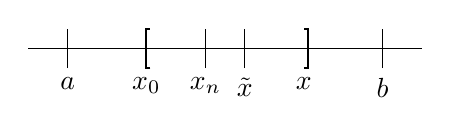
\begin{tikzpicture}[scale=0.5]
\draw (-1,0)-- (9,0); %Axis

\draw (0,-.5) -- (0,.5);
\draw (0,-0.5) node[anchor=north] {$a$};

\draw [thick] (2.1,-.5) -- (2,-.5) -- (2,.5) -- (2.1,.5); 
\draw (2,-.5) node [anchor=north] {$x_0$};

\draw (3.5,-.5) -- (3.5,.5);
\draw (3.5,-0.5) node[anchor=north] {$x_n$};

\draw (4.5,-.5) -- (4.5,.5);
\draw (4.5,-0.5) node[anchor=north] {$\tilde{x}$};

\draw [thick] (6,-.5) -- (6.1,-.5) -- (6.1,.5) -- (6,.5); 
\draw (6,-.5) node [anchor=north] {$x$};

\draw (8,-.5) -- (8,.5);
\draw (8,-0.5) node[anchor=north] {$b$};

\end{tikzpicture}
\end{center}

\begin{enumerate}[-]
\item Si $x\notin[x_0,\tilde{x}] \Rightarrow x\notin [x_0,x_n]$ para $n\geq n_0$.
\item Si $x\in(x_0,\tilde{x}) \Rightarrow x\in [x_0,x_n]$ para $n\geq n_0$.
\end{enumerate}

Y ese es la clave que nos va a permitir ver que $f(x_n)\to f(\tilde{x})$. Sea $J$ un intervalo compacto de forma que $[x_0,x]\subset J\subset(a,b)$.

\[
\integral{x_0}{x_n}{g(x)dx}=\integral{J}{}{g(x)\chi_{[x_0,x_n]}}(x)dx
\]

Usando lo anterior obtenemos la convergencia puntual de la sucesión $g(x)\chi_{[x_0,x_n]}\overset{cp}{\longrightarrow}g(x)\chi_{(x_0,\tilde{x})}$. Lo que nos da la convergencia en integral también:

\[
f(x_n)=\integral{J}{}{g(x)\chi_{[x_0,x_n]}(x)dx}\overset{cp}{\longrightarrow}\integral{J}{}{g(x)\chi_{(x_0,\tilde{x})}(x)dx}=\integral{x_0}{\tilde{x}}{g(x)dx}=f(\tilde{x})
\]

Luego $f\in C(a,b) \Rightarrow f\in \localmenteintegrable$.

Ahora nos queda ver $f'=g$. Para ello tenemos que comprobar que:

\[
\integral{a}{b}{f(x)\phi'(x)dx}+\integral{a}{b}{g(x)\phi(x)dx}=0 \espacio \forall \phi\in \soportecompacto
\]

Tenemos el problema de que $g$ no tiene por qué ser derivable (podría ser una función escalón, por ejemplo). Vamos a empezar suponiendo que $g\in L^1([a,b])$ (para que $f$ esté bien definida) y que $x_0=a$. Al final reduciremos esas hipótesis hasta llegar a que $g\in\localmenteintegrable$.

\underline{Paso 1}: $g\in L^1([a,b])$ y $x_0=a$. Para ver que
\[
\integral{a}{b}{f(x)\phi'(x)dx}=-\integral{a}{b}{g(x)\phi(x)dx} 
\]

vamos a tener que usar el Teorema de Fubini-Tonelli.

\[
\integral{a}{b}{f(x)\phi'(x)dx}=
\integral{a}{b}{\left(\integral{a}{x}{g(s)ds}\right)\phi'(x)dx}\overset{TªFT}{=}
\integral{a}{b}{\left(\integral{s}{b}{g(s)\phi'(x)dx}\right)ds}=\]
\[
\integral{a}{b}{g(s)\left(\integral{s}{b}{\phi'(x)dx}\right)ds}
=\integral{a}{b}{g(s)(\underbrace{\phi(b)}_{=0}-\phi(s))ds}=-\integral{a}{b}{g(s)\phi'(s)ds}
\]

\underline{Paso 2}: Reemplazamos la hipótesis $x_0=a$ por $x_0\in(a,b)$ y usamos el paso 1:

\[
\integral{a}{b}{g(x)\phi(x)dx}=-\integral{a}{b}{\left(\integral{a}{x}{g(s)ds}\right)\phi'(x)dx}
\]

Vemos que la integral del interior se puede expresar como una constante más una función:

\[
\integral{a}{x}{g(s)ds}=\underbrace{\integral{a}{x_0}{g(s)ds}}_{cte=C}+\underbrace{\integral{x_0}{x}{g(s)ds}}_{funcion}
\]

Luego:

\[
-\integral{a}{b}{\left(\integral{a}{x}{g(s)ds}\right)\phi'(x)dx}=
-\underbrace{\integral{a}{b}{B\phi'(x)dx}}_{=B(\phi(b)-phi(a))=0}-\integral{a}{b}{\left(\integral{x_0}{x}{g(s)ds}\right)\phi'(x)dx}=
-\integral{a}{b}{f(x)\phi(x)dx}
\]

\underline{Caso 3}: Ahora sustituimos la hipótesis $g\in L^1([a,b])$ por $g\in\localmenteintegrable$. Tomamos un subintervalo compacto $[a'.b']\subset(a,b)$ donde $g_{|[a'.b']}\in L^1([a',b'])$, de forma que $\supp\phi\subset[a',b']$. Sea $x_0\in[a',b']$ y $x\in(a,b)$.

Ahora aplicamos el caso 2, usando que $\supp\phi\subset[a',b']$:

\[
\integral{a}{b}{g(x)\phi(x)dx}=\integral{a'}{b'}{g(x)\phi(x)dx}=-\integral{a'}{b'}{\left(\integral{x_0}{x}{g(s)ds}\right)\phi'(x)dx}=-\integral{a}{b}{f(x)\phi'(x)dx}
\]

\end{proof}
